\section{Installing \LaTeX}
Thre are two main options: TeX Live and MiKTeX, both put together all the underlying components that are necessary to create documents, and both exist in all operating systems.
However, below you can see the recommendations and direct links to get you started.

\subsection{Windows}
Download MiKTeX on this \href{https://miktex.org/download}{link}.
It even includes step-by-step instructions for the installation wizard, if you so require.

\subsection{Mac}
For both Mac and Linux the suggestion is to use variations of TeXlive.  
\href{https://www.tug.org/texlive/}{Link} to all the instructions.
The web page is pure text, so the navigation can be a little challenging.
Below is some information which links to the appropriate area.

To install MacTeX, follow the instructions \href{https://www.tug.org/mactex/mactex-download.html}{link}

MacTeX will install TeX Live, plus a few other utilities.
Either of the suggested editors will still need to be installed.  

\subsection{Linux}
Your package manager will have a TeX Live distribution. \href{https://wiki.archlinux.org/title/TeX_Live}{Link} to the Arch Linux wiki.

Fedora and other RPM based distributions can download it with
\begin{lstlisting}
    # dnf install texlive-scheme-full
\end{lstlisting}

Debian/Ubuntu:
\begin{lstlisting}
    # apt-get install texlive
\end{lstlisting}

\section{Installing an IDE}
\subsection{Visual Studio Code}
\href{https://code.visualstudio.com/}{Download}

VSCode is a general purpose editor, and if you plan on doing any programming at all, it may be worth becoming more familiar with it.
Microsoft has an excellent introduction to it in their \href{https://code.visualstudio.com/docs}{website}.

In order to give VSCode the ability to work with and compile \LaTeX{}, we must install the LaTeX Workshop extension.
Start by opening the extensions on the side bar (shortcut: \texttt{ctrl+shift+x}).
Search for ``latex'' and the first option should be LaTeX Workshop published by James Yu.

\begin{figure}[h]
\centering
    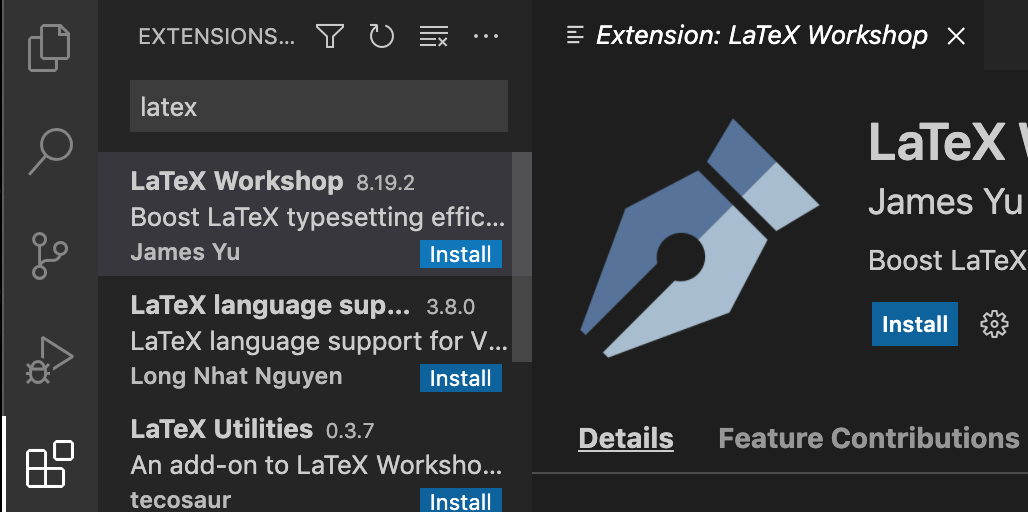
\includegraphics[width=0.65\textwidth]{figures/extension.png}
\label{fig:extension}
\caption{Installing LaTeX Workshop}
\end{figure}

\subsubsection{Editor settings}
Feel free to play around with the settings, themes, etc to find what you like, but there is one specific setting that is an absolute must:
disabling ``Snippets Prevent Quick Suggestions''.

To do so, open the settings with \texttt{ctrl + ,} (Mac: \texttt{cmd + ,}), search for \texttt{editor.suggest.snippets}, and disable it/set it to false.

\begin{figure}[h]
\centering
    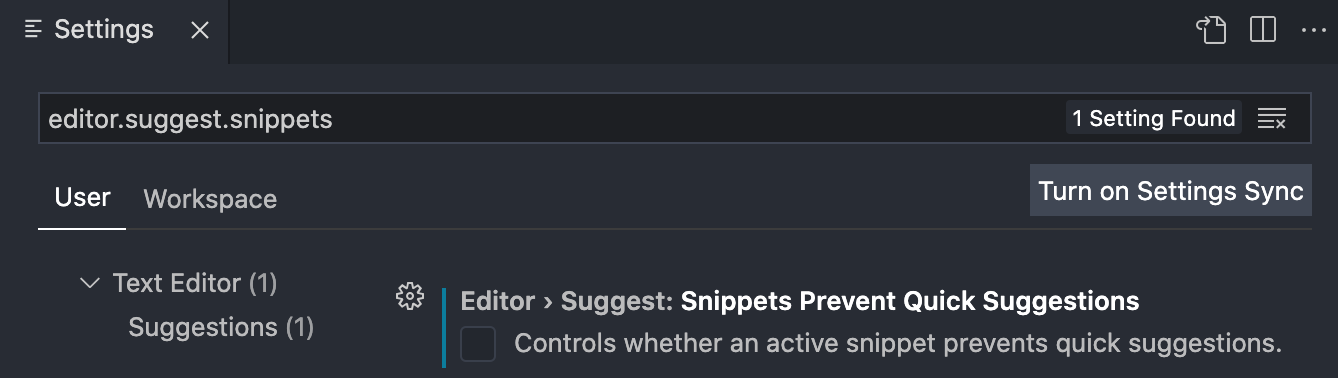
\includegraphics[width=0.8\textwidth]{figures/quick-suggests.png}
    \label{fig:quick-suggests}
    \caption{Disabling Snippets Prevent Quick Suggestions}
\end{figure}

\subsubsection{Compilation}
Unless changed in the settings, your \texttt{.tex} will be compiled on saving the file.
If compilation on save does not trigger, you can manually do it with a few different options:
\begin{enumerate}
    \item Open the command pallet (\verb|ctrl+shift+P|), type ``latex build'' and select the option ``LaTeX Workshop: Build LaTeX Project''
    \item On the top right, while in a \texttt{.tex} file, click the green arrow (\texttt{ctrl+alt+B}).
    \begin{figure}[h]
    \centering
        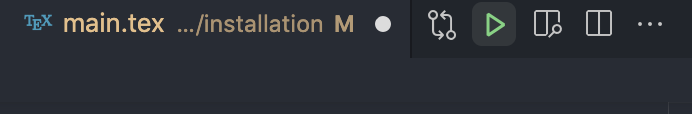
\includegraphics[width=0.6\textwidth]{figures/build.png}
    \label{fig:build}
    \caption{Manually building LaTeX project}
    \end{figure}
\end{enumerate} 

\subsubsection{LaTeX Workshop}
The LaTeX Workshop extension should also give you access to another tab on the left-hand side.
This includes navigating the document's structure and seeing helpful math symbols.
\begin{figure}[h]
\centering
    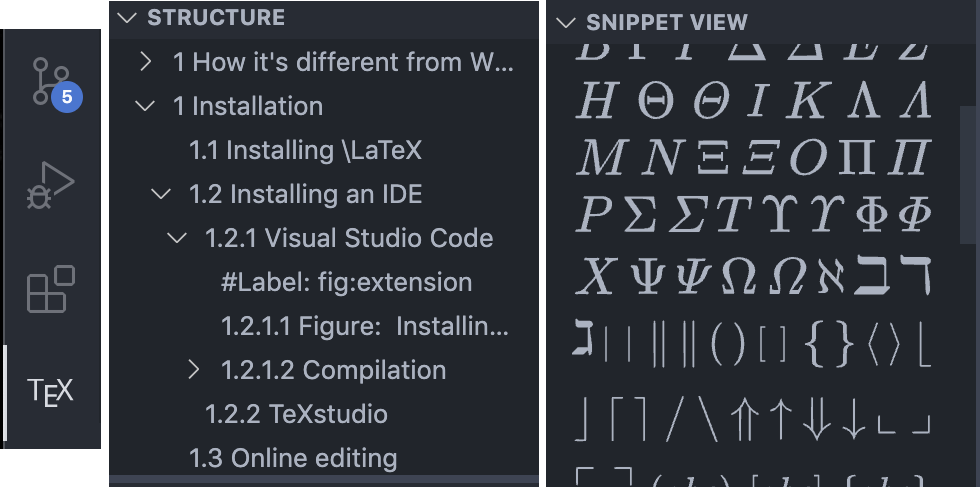
\includegraphics[width=0.7\textwidth]{figures/symbols.png}
\label{fig:symbols}
\caption{Accessing useful tools provided by LaTeX Workshop}
\end{figure}

\subsection{TeXstudio}
\href{https://www.texstudio.org/}{Download}

TeXstudio is an IDE dedicated to \LaTeX{}, so there is minimal setup. Simply download and you're ready to go!

If you really like interacting with a graphical interface, it is hard to go wrong with TeXstudio.
Throughout this document we will focus on generating it all with text using VSCode, but TeXstudio can do it all, and it provides tools to help generate tables, include graphics, initiate documents, etc.

\section{Online editing}
If you need a tool similar to Google Drive/One Drive for online collaboration, the most popular option is \href{https://www.overleaf.com/}{Overleaf}.
UCL students and staff have access to professional accounts on Overleaf, and the link to activate it can be found in the software database: \href{https://swdb.ucl.ac.uk/package/view/id/1235}{here}.